% =========================================================================
% Dynamic EMS Dispatch & Station Placement Optimization -- review deck
%
% Shares paper/figures/ with main.tex, so every chart here is the one the
% paper prints and the app renders -- same models, same colour tokens, drawn
% by paper/make_figures.py. Rebuild figures first if the data changes:
%
%     python paper/make_figures.py
%     pdflatex -output-directory=paper paper/slides.tex   (twice, for slide totals)
%
% Theme is hand-rolled rather than metropolis: BasicTeX ships neither
% metropolis nor the Fira/Lato families it wants, and a deck that fails to
% build on the machine it is presented from is worse than a plain one.
% =========================================================================
\documentclass[aspectratio=169,10pt]{beamer}

\usepackage[T1]{fontenc}
\usepackage[utf8]{inputenc}
% No helvet / lmodern / Fira here. BasicTeX ships helvet.sty but not the
% Helvetica metrics (phvr8t.tfm), so loading it is a hard build failure on a
% stock install. Beamer's own Computer Modern Sans is present everywhere and
% is what this deck is set in.
\usepackage{amsmath,amssymb}
\usepackage{booktabs}
\usepackage{graphicx}
\usepackage{tikz}
% microtype omitted deliberately: its font expansion requires scalable fonts,
% and with BasicTeX's bitmap Computer Modern it is a fatal error, not a
% degraded result.
\usepackage{xcolor}

\graphicspath{{figures/}{paper/figures/}}

% --- palette: the src/viz.py tokens, so deck, paper and app are one system
\definecolor{inkp}{HTML}{0B0B0B}   % primary text
\definecolor{inks}{HTML}{52514E}   % secondary text
\definecolor{inkm}{HTML}{8A8985}   % muted
\definecolor{rule}{HTML}{E4E3DF}   % hairlines
\definecolor{s1}{HTML}{2A78D6}     % slot 1 -- always "our optimised result"
\definecolor{s2}{HTML}{EB6834}     % slot 2 -- always "the existing/benchmark"
\definecolor{s3}{HTML}{1BAF7A}
\definecolor{good}{HTML}{008300}

\setbeamercolor{normal text}{fg=inkp}
\setbeamercolor{frametitle}{fg=inkp}
\setbeamercolor{structure}{fg=s1}
\setbeamercolor{itemize item}{fg=s1}
\setbeamercolor{itemize subitem}{fg=inkm}
\setbeamercolor{alerted text}{fg=s2}

\setbeamerfont{frametitle}{size=\large,series=\bfseries}
\setbeamerfont{framesubtitle}{size=\small,series=\mdseries}
\setbeamercolor{framesubtitle}{fg=inks}
\setbeamerfont{title}{size=\LARGE,series=\bfseries}

\setbeamertemplate{navigation symbols}{}
\setbeamertemplate{itemize item}{\textbullet}
\setbeamertemplate{itemize subitem}{--}

% Frametitle with a hairline under it: the only chrome on the slide.
%
% Built from \par + \vspace rather than \\. A beamer frametitle template is
% expanded in vertical mode, where \\ raises "There's no line here to end" on
% every single frame -- the deck still produced a PDF, which is exactly what
% makes that class of error easy to ship by accident. \@empty also needs
% \makeatletter here, since the template lives in the document preamble.
\makeatletter
\setbeamertemplate{frametitle}{%
  \vspace{0.6em}%
  \begin{minipage}{\textwidth}%
    \raggedright
    \usebeamerfont{frametitle}\usebeamercolor[fg]{frametitle}\insertframetitle\par
    \ifx\insertframesubtitle\@empty\else
      \vspace{0.15em}%
      \usebeamerfont{framesubtitle}\usebeamercolor[fg]{framesubtitle}%
      \insertframesubtitle\par
    \fi
    \vspace{0.35em}%
    {\color{rule}\rule{\textwidth}{0.6pt}}%
  \end{minipage}%
}
\makeatother

% A full-width hairline that is safe in both horizontal and vertical mode,
% so section breaks inside a frame cannot reintroduce the bug above.
\newcommand{\hairline}[1][0.6em]{%
  \par\vspace{0.3em}\noindent{\color{rule}\rule{\textwidth}{0.6pt}}\par\vspace{#1}%
}

% Wrapped in a sized, right-aligned box. A bare \hspace*{\fill} in a footline
% template has no bounding box to align against, so the trailing content runs
% off the right paper edge and the last glyph is clipped -- silently, with no
% overfull warning, because the template is never measured as a paragraph.
\setbeamertemplate{footline}{%
  \begin{beamercolorbox}[wd=\paperwidth,ht=2.6ex,dp=1.4ex,right]{}%
    \scriptsize\color{inkm}%
    EMS dispatch \& station placement\quad\textbar\quad%
    \insertframenumber/\inserttotalframenumber%
    \hspace{1.6em}%
  \end{beamercolorbox}%
}

% A number worth saying out loud, for the result slides.
\newcommand{\stat}[2]{{\color{s1}\textbf{#1}}\ {\footnotesize\color{inks}#2}}
% Inline caveat, used wherever a figure could be over-read.
\newcommand{\caveat}[1]{{\footnotesize\color{inks}\textit{#1}}}

\title{Dynamic EMS Dispatch \&\\Station Placement Optimization}
\subtitle{Integrated station siting and ambulance dispatch\\on 2.2 million Seattle 911 records}
\author{Aadith Krishna \and Aditya Santosh \and Suryansh Ram Menon \and Arjun Gopal}
\date{Operations Research --- Final Review}

\begin{document}

% =========================================================================
\begin{frame}[plain]
  \vspace{1.2em}
  {\usebeamerfont{title}\color{inkp}\inserttitle\par}
  \vspace{0.7em}{\color{rule}\rule{0.45\textwidth}{1.2pt}}\par
  \vspace{0.7em}
  {\large\color{inks}Integrated station siting and ambulance dispatch\\
   on \textbf{2.2 million} real Seattle 911 records\par}
  \vspace{1.6em}
  {\footnotesize\color{inks}%
   Aadith Krishna \textit{(CB.SC.U4AIE23202)} \quad
   Aditya Santosh \textit{(CB.SC.U4AIE23207)}\\[0.25em]
   Suryansh Ram Menon \textit{(CB.SC.U4AIE23255)} \quad
   Arjun Gopal \textit{(CB.SC.U4AIE23271)}\par}
  \vspace{1.0em}
  {\footnotesize\color{inkm}Operations Research \ \textbar\ \ Final Review\par}
\end{frame}

% =========================================================================
\begin{frame}{Survival is decided in minutes}{Two operational decisions control how fast an ambulance arrives}
  \vspace{0.6em}
  \begin{columns}[T,onlytextwidth]
    \begin{column}{0.47\textwidth}
      {\color{s1}\textbf{\large Q1 \ --- \ Where should ambulances wait?}}\\[0.5em]
      {\color{inks}Place stations well and more of the city sits inside a short
       response radius. A \emph{strategic} decision, made once.}\\[0.9em]
      {\footnotesize\color{inkm}Set covering / maximal covering --- ILP}
    \end{column}
    \begin{column}{0.47\textwidth}
      {\color{s2}\textbf{\large Q2 \ --- \ Who should be sent?}}\\[0.5em]
      {\color{inks}When several emergencies land at once, the right
       ambulance-to-incident matching cuts everyone's wait. An
       \emph{operational} decision, made every hour.}\\[0.9em]
      {\footnotesize\color{inkm}Assignment problem --- LP}
    \end{column}
  \end{columns}
  \vspace{1.3em}
  \hairline[0.6em]
  \centering
  \textbf{The two are linked:} the stations chosen by the covering model
  \emph{become} the ambulance bases the assignment model dispatches from.
\end{frame}

% =========================================================================
\begin{frame}{The pipeline}{Five stages, each one feeding the next}
  \vspace{0.4em}
  \centering
  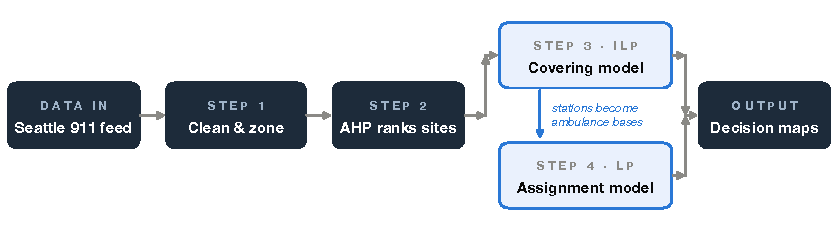
\includegraphics[width=0.96\textwidth]{fig1_pipeline.pdf}
  \vspace{0.6em}
  \begin{columns}[T,onlytextwidth]
    \begin{column}{0.49\textwidth}
      {\footnotesize\color{inks}%
      Every stage runs on the real feed. No synthetic demand, no sampled
      subset, no hand-picked study area.}
    \end{column}
    \begin{column}{0.49\textwidth}
      {\footnotesize\color{inks}%
      All three models solve locally in milliseconds --- the whole pipeline is
      interactive, not a batch job.}
    \end{column}
  \end{columns}
\end{frame}

% =========================================================================
\begin{frame}{The data}{Three public sources, no API keys, fully reproducible}
  \vspace{0.3em}
  \centering
  {\footnotesize
  \begin{tabular}{@{}lll@{}}
    \toprule
    \textbf{Source} & \textbf{What it is} & \textbf{Used for} \\
    \midrule
    Seattle Real-Time Fire 911 Calls & 2,197,739 records, 2003--2026 & Where and when emergencies occur \\
    Seattle Fire Stations (City GIS) & The 36 stations Seattle runs    & Benchmarking our placement \\
    ZIP Code Tabulation Areas (Census) & ZIP polygons                  & Assigning each incident a zone \\
    \bottomrule
  \end{tabular}}
  \vspace{1.1em}

  \begin{columns}[T,onlytextwidth]
    \begin{column}{0.3\textwidth}\centering
      \stat{79,152}{EMS incidents}\\{\scriptsize\color{inkm}study year, 27 Aug 2025 -- 27 Aug 2026}
    \end{column}
    \begin{column}{0.3\textwidth}\centering
      \stat{28}{demand zones}\\{\scriptsize\color{inkm}after a materiality floor}
    \end{column}
    \begin{column}{0.3\textwidth}\centering
      \stat{36}{real stations}\\{\scriptsize\color{inkm}the benchmark network}
    \end{column}
  \end{columns}
  \vspace{1.0em}
  \centering\caveat{The raw feed mixes fire, alarms and hazmat with EMS;
  calls are filtered to genuine aid/medic dispatches by whole-word patterns,
  de-duplicated on incident number, and tagged by point-in-polygon join.}
\end{frame}

% =========================================================================
\begin{frame}{Step 1 --- Demand is concentrated, not uniform}{Which is exactly why placement can beat history}
  \vspace{0.2em}
  \begin{columns}[c,onlytextwidth]
    \begin{column}{0.56\textwidth}
      \centering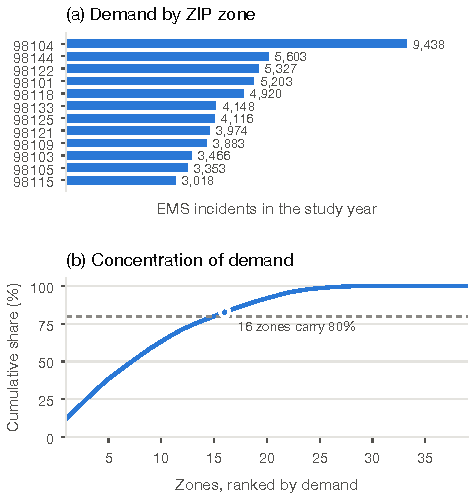
\includegraphics[height=0.66\textheight]{fig2_demand.pdf}
    \end{column}
    \begin{column}{0.4\textwidth}
      {\color{inks}The 15 busiest ZIP zones carry \textbf{\color{s1}80.0\%} of
      all 79,152 incidents.}\\[0.9em]
      {\color{inks}Zone 98104 alone accounts for \textbf{9,438} calls ---
      11.9\% of the city's EMS demand in one ZIP.}\\[0.9em]
      {\footnotesize\color{inkm}Each zone becomes a demand point weighted by
      its incident count, located at the \emph{mean incident coordinate}
      rather than the polygon centroid --- the candidate site sits where the
      calls actually are.}
    \end{column}
  \end{columns}
\end{frame}

% =========================================================================
\begin{frame}{Step 1 --- When the load spikes}{A midday peak, and a flat week}
  \vspace{0.2em}
  \centering
  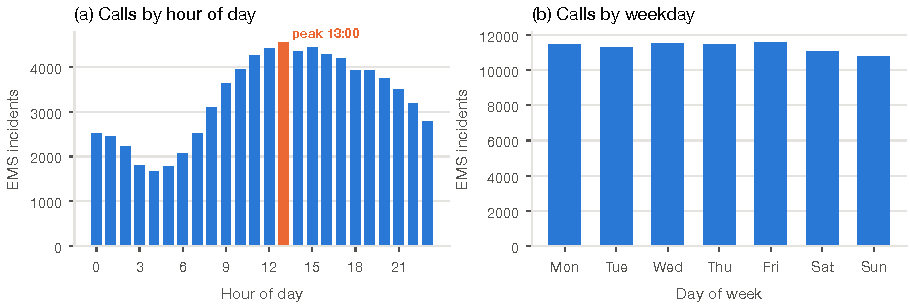
\includegraphics[width=0.92\textwidth]{fig3_temporal.pdf}
  \vspace{0.4em}

  {\footnotesize\color{inks}Demand peaks at \textbf{13:00} and runs roughly
  \textbf{216 calls/day}. The weekday spread is only a few percent
  (Fri 11,577 against Sun 10,757), so the \emph{hour} matters for dispatch
  while the \emph{day} does not --- which is why the dispatch scenario is
  chosen by peak hour, not by weekday.}
\end{frame}

% =========================================================================
\begin{frame}{Step 2 --- AHP: turning three competing criteria into one score}
  \vspace{0.4em}
  \begin{columns}[T,onlytextwidth]
    \begin{column}{0.46\textwidth}
      {\footnotesize
      \begin{tabular}{@{}ll@{}}
        \toprule
        \textbf{Criterion} & \textbf{Weight} \\
        \midrule
        Incident Density    & \textbf{\color{s1}67.4\%} \\
        Equity Gap          & 23.1\% \\
        Coverage Potential  & \phantom{0}9.4\% \\
        \bottomrule
      \end{tabular}}\\[1.0em]
      {\footnotesize\color{inks}Four members rate the three criteria pairwise
      on Saaty's 1--9 scale, independently. Matrices are combined by
      \textbf{element-wise geometric mean} --- the only average that keeps the
      matrix reciprocal.}
    \end{column}
    \begin{column}{0.5\textwidth}
      {\color{inks}Weights are the principal eigenvector. Human judgements can
      quietly contradict each other, so AHP measures that:}\\[0.6em]
      \centering
      $\mathrm{CI}=\dfrac{\lambda_{\max}-n}{n-1}, \qquad
       \mathrm{CR}=\dfrac{\mathrm{CI}}{\mathrm{RI}}$\\[0.9em]
      \begin{tabular}{@{}llll@{}}
        \toprule
        $\lambda_{\max}$ & CI & RI & CR \\
        \midrule
        3.0000 & 0.0000 & 0.58 & \textbf{\color{good}0.0000} \\
        \bottomrule
      \end{tabular}\\[0.7em]
      {\footnotesize\color{good}$\mathrm{CR}<0.10$ for all four members
      \emph{individually} and for the aggregate.}
    \end{column}
  \end{columns}
  \vspace{0.6em}
  \caveat{CR is exactly zero by construction, not by luck: each member's
  density-vs-coverage rating is the product of their other two, so the
  judgements contain no contradiction for the check to find.}
\end{frame}

% =========================================================================
\begin{frame}{Step 3 --- Optimisation 1: where to put the stations}
  \vspace{0.3em}
  \begin{columns}[T,onlytextwidth]
    \begin{column}{0.48\textwidth}
      {\color{s1}\textbf{Mode A --- Set covering}}\\
      {\footnotesize\color{inks}Fewest stations that put \emph{every} zone in reach.}\\[0.4em]
      \begin{align*}
        \min\ & \textstyle\sum_i y_i \\
        \text{s.t.}\ & \textstyle\sum_{i \in N(j)} y_i \ \geq\ 1 \quad \forall j \\
                     & y_i \in \{0,1\}
      \end{align*}
    \end{column}
    \begin{column}{0.48\textwidth}
      {\color{s2}\textbf{Mode B --- Maximal covering}}\\
      {\footnotesize\color{inks}On a fixed budget $P$, cover the most \emph{demand}.}\\[0.4em]
      \begin{align*}
        \max\ & \textstyle\sum_j d_j z_j \\
        \text{s.t.}\ & z_j \ \leq\ \textstyle\sum_{i \in N(j)} y_i \quad \forall j \\
                     & \textstyle\sum_i y_i = P, \quad y_i, z_j \in \{0,1\}
      \end{align*}
    \end{column}
  \end{columns}
  \vspace{0.5em}
  \hairline[0.5em]
  {\footnotesize\color{inks}$N(j)$ is the set of candidate sites that reach
  zone $j$ inside the limit; $d_j$ is the zone's incident count, so Mode B
  maximises \emph{people reached}, not area or zone count. Solved exactly with
  HiGHS via PuLP --- \textbf{5\,ms} on the study instance.}
\end{frame}

% =========================================================================
\begin{frame}{Step 3 --- The eight-minute solution}
  \vspace{0.2em}
  \begin{columns}[c,onlytextwidth]
    \begin{column}{0.5\textwidth}
      \centering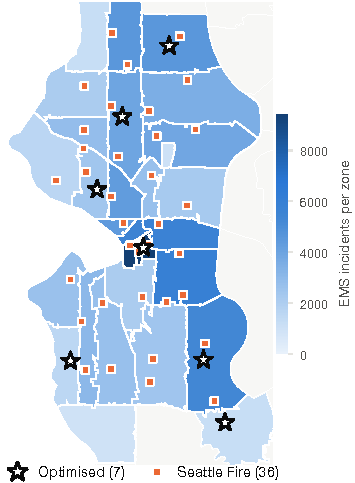
\includegraphics[height=0.70\textheight]{fig4_map.pdf}
    \end{column}
    \begin{column}{0.46\textwidth}
      \stat{7}{stations}\\[0.3em]
      \stat{100.0\%}{of demand covered}\\[0.3em]
      \stat{28/28}{zones inside 8 minutes}\\[0.3em]
      \stat{5\,ms}{to prove optimality}\\[1.0em]
      {\footnotesize\color{inks}Against Seattle's \textbf{36} real stations at
      the same limit.}\\[0.7em]
      {\footnotesize\color{s2}\textbf{But hold that number} --- the next slide
      is why \emph{7} should never be quoted on its own.}
    \end{column}
  \end{columns}
\end{frame}

% =========================================================================
\begin{frame}{How much of this is Seattle, and how much is our assumption?}{The slide we would want a reviewer to ask for}
  \vspace{0.2em}
  \begin{columns}[c,onlytextwidth]
    \begin{column}{0.47\textwidth}
      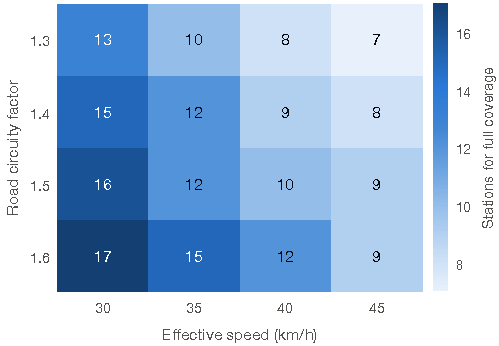
\includegraphics[width=\textwidth]{fig8_robustness.pdf}
    \end{column}
    \begin{column}{0.49\textwidth}
      {\footnotesize\color{inks}The 911 feed records \textbf{no response
      times}. Every minute in this project is computed:}\\[0.4em]
      \centering{\footnotesize $t = \dfrac{d_{\text{haversine}} \times
       \text{circuity}}{\text{speed}} + \text{turnout}$}\\[0.8em]
      \raggedright
      {\footnotesize\color{inks}So we re-solved the ILP across a $4\times4$
      grid of those two constants --- 16 exact solves.}\\[0.8em]
      \stat{7--17}{stations, a 2.4$\times$ spread}\\[0.3em]
      \stat{100\%}{coverage in \emph{all} 16 cells}
    \end{column}
  \end{columns}
  \vspace{0.7em}
  \hairline[0.5em]
  \centering
  \textbf{The count is assumption-dependent. Being under 36 is not.}
\end{frame}

% =========================================================================
\begin{frame}{Step 3 --- What a tighter promise costs}
  \vspace{0.2em}
  \begin{columns}[c,onlytextwidth]
    \begin{column}{0.5\textwidth}
      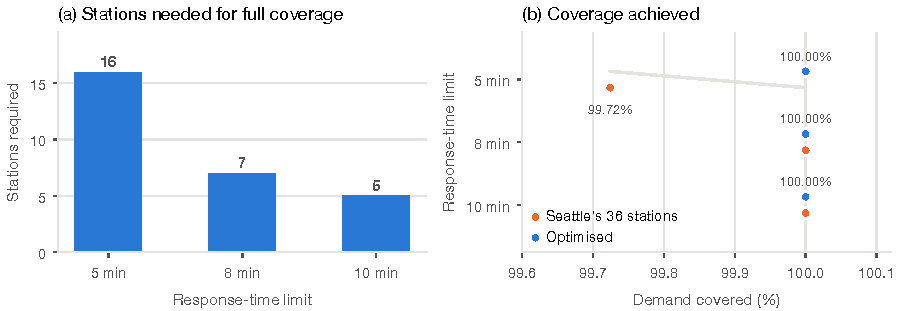
\includegraphics[width=\textwidth]{fig6_sweep.pdf}\\
      \centering{\scriptsize\color{inkm}Stations needed per response limit}
    \end{column}
    \begin{column}{0.46\textwidth}
      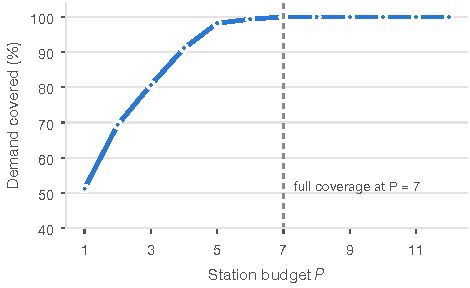
\includegraphics[width=\textwidth]{fig5_curve.pdf}\\
      \centering{\scriptsize\color{inkm}Diminishing returns against budget $P$}
    \end{column}
  \end{columns}
  \vspace{0.5em}
  {\footnotesize\color{inks}Tightening the promise from 10 to 5 minutes takes
  the network from \textbf{5} stations to \textbf{16} --- the cost of a
  guarantee is convex. The budget curve is the argument for Mode B: the first
  handful of stations buy most of the city, and the last few buy very little.}
\end{frame}

% =========================================================================
\begin{frame}{Step 3 --- Against the network Seattle actually runs}
  \vspace{0.3em}
  \centering
  {\footnotesize
  \begin{tabular}{@{}lccc@{}}
    \toprule
    \textbf{Response limit} & \textbf{Our stations} & \textbf{Demand covered} & \textbf{Seattle's 36} \\
    \midrule
    \phantom{0}5 min & 16 & 100\% & 99.72\% \\
    \phantom{0}8 min & \textbf{\color{s1}7} & 100\% & 100\% \\
    10 min & \phantom{0}5 & 100\% & 100\% \\
    \bottomrule
  \end{tabular}}
  \vspace{1.1em}

  \begin{columns}[T,onlytextwidth]
    \begin{column}{0.48\textwidth}
      {\color{good}\textbf{What this supports}}\\[0.3em]
      {\footnotesize\color{inks}Placement that follows \emph{measured demand}
      reaches the whole city from fewer sites than placement accumulated
      historically. Directionally true in every cell of the robustness grid.}
    \end{column}
    \begin{column}{0.48\textwidth}
      {\color{s2}\textbf{What it does not}}\\[0.3em]
      {\footnotesize\color{inks}The 36 are \emph{fire} stations --- they also
      carry suppression, hazmat and technical rescue, missions this model does
      not place for. The comparison is not like-for-like, and the ratio
      flatters us.}
    \end{column}
  \end{columns}
\end{frame}

% =========================================================================
\begin{frame}{Step 4 --- Optimisation 2: who to send}
  \vspace{0.4em}
  \begin{columns}[T,onlytextwidth]
    \begin{column}{0.44\textwidth}
      \begin{align*}
        \min\ & \textstyle\sum_i \sum_j c_{ij}\, x_{ij} \\
        \text{s.t.}\ & \textstyle\sum_i x_{ij} = 1 \quad \forall j \\
                     & \textstyle\sum_j x_{ij} \leq 1 \quad \forall i \\
                     & x_{ij} \geq 0
      \end{align*}
      {\footnotesize\color{inks}$c_{ij}$ is travel time from ambulance $i$ to
      incident $j$. The constraint matrix is totally unimodular, so the LP
      relaxation is integral --- no branching needed.}
    \end{column}
    \begin{column}{0.52\textwidth}
      {\color{inks}\textbf{Scenario:} the busiest hour in the study year ---
      Wed 19 Nov 2025, 09:00, \textbf{30 simultaneous incidents}, dispatched
      from the \textbf{7 stations the covering model opened}.}\\[0.8em]
      {\footnotesize\color{inks}A rectangular cost matrix is padded with
      zero-cost dummy rows or columns so the problem is square and balanced;
      dummies never distort the real total.}\\[0.8em]
      {\footnotesize\color{inkm}Cross-checked against an independent
      Hungarian-algorithm solution: identical to six decimal places.}
    \end{column}
  \end{columns}
\end{frame}

% =========================================================================
\begin{frame}{Step 4 --- Optimal dispatch against nearest-unit-first}
  \vspace{0.2em}
  \begin{columns}[c,onlytextwidth]
    \begin{column}{0.45\textwidth}
      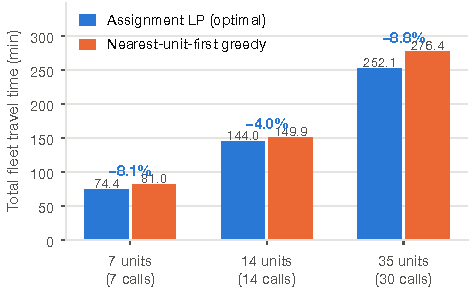
\includegraphics[width=\textwidth]{fig7_dispatch.pdf}
    \end{column}
    \begin{column}{0.51\textwidth}
      {\footnotesize
      \begin{tabular}{@{}lrrr@{}}
        \toprule
        \textbf{Fleet} & \textbf{Optimal} & \textbf{Greedy} & \textbf{Gain} \\
        \midrule
        35 units \textit{(default)} & 252.1 & 276.4 & \textbf{\color{s1}8.8\%} \\
        14 units & 144.0 & 149.9 & 4.0\% \\
        \phantom{0}7 units & \phantom{0}74.4 & \phantom{0}81.0 & 8.1\% \\
        \bottomrule
      \end{tabular}}\\[0.9em]
      {\footnotesize\color{inks}\textbf{Both sides clear the same calls.}
      A peak hour has more calls than units, and unserved calls cost nothing
      in the objective --- so an unrestricted LP would quietly answer only the
      \emph{nearest} calls while greedy took them as they came.}\\[0.5em]
      {\footnotesize\color{s2}Comparing those totals would score \emph{triage}
      rather than \emph{routing} and inflate our margin to 62\%.}
    \end{column}
  \end{columns}
\end{frame}

% =========================================================================
\begin{frame}{What is measured, and what is modelled}{Stated before it is asked}
  \vspace{0.5em}
  \begin{columns}[T,onlytextwidth]
    \begin{column}{0.48\textwidth}
      {\color{good}\textbf{Measured}}\\[0.5em]
      {\footnotesize\color{inks}
      $\bullet$\ Incident locations, times and counts --- 2.2M actual records\\[0.35em]
      $\bullet$\ The 36 real station locations\\[0.35em]
      $\bullet$\ ZIP zone geometry\\[0.35em]
      $\bullet$\ Every optimisation result, solved exactly and verified}
    \end{column}
    \begin{column}{0.48\textwidth}
      {\color{s2}\textbf{Modelled}}\\[0.5em]
      {\footnotesize\color{inks}
      $\bullet$\ \textbf{Every response time} --- the feed contains none\\[0.35em]
      $\bullet$\ Demand aggregated to 28 zone centroids\\[0.35em]
      $\bullet$\ AHP weights --- subjective by design, hence the CR test\\[0.35em]
      $\bullet$\ Units assumed always free (no queueing)}
    \end{column}
  \end{columns}
  \vspace{1.0em}
  \hairline[0.6em]
  {\footnotesize\color{inks}This is an optimisation over \textbf{real demand
  geography} with a \textbf{modelled travel layer}. Its claims are therefore
  comparative --- which sites, in what order, how the answer moves --- rather
  than predictive. Which is why the robustness grid is a result slide and not
  an appendix.}
\end{frame}

% =========================================================================
\begin{frame}{Verification --- the models are not taken on trust}
  \vspace{0.4em}
  \begin{columns}[T,onlytextwidth]
    \begin{column}{0.49\textwidth}
      {\footnotesize\color{inks}
      $\bullet$\ Set covering matched \textbf{brute force} on 25 fully
      enumerated instances\\[0.4em]
      $\bullet$\ Maximal covering matched brute force on 25 instances\\[0.4em]
      $\bullet$\ AHP weights matched the largest-modulus eigenvector on
      \textbf{200 random matrices}\\[0.4em]
      $\bullet$\ Optimal dispatch never lost to greedy over \textbf{150 random
      cost matrices}\\[0.4em]
      $\bullet$\ Assignment LP matched an independent \textbf{Hungarian}
      solution exactly}
    \end{column}
    \begin{column}{0.47\textwidth}
      \centering
      \vspace{0.4em}
      \stat{64}{model checks}\\[0.5em]
      \stat{31}{application tests}\\[0.5em]
      \stat{0}{failures}\\[1.0em]
      {\footnotesize\color{inks}Including monotonicity of the robustness grid:
      a slower fleet or twistier roads can never need \emph{fewer}
      stations --- which is what separates a real gradient from solver noise.}
    \end{column}
  \end{columns}
\end{frame}

% =========================================================================
\begin{frame}{It is a live application, not a script}
  \vspace{0.6em}
  \begin{columns}[T,onlytextwidth]
    \begin{column}{0.5\textwidth}
      {\color{inks}Four tabs, every model re-solving interactively:}\\[0.6em]
      {\footnotesize\color{inks}
      $\bullet$\ \textbf{Data} --- demand in space and time\\[0.3em]
      $\bullet$\ \textbf{Site scoring} --- AHP, live Saaty sliders\\[0.3em]
      $\bullet$\ \textbf{Station placement} --- both ILP modes, sensitivity,
      robustness, benchmark\\[0.3em]
      $\bullet$\ \textbf{Dispatch} --- the LP on any peak hour}
    \end{column}
    \begin{column}{0.46\textwidth}
      {\color{inks}Every assumption is a control, not a constant:}\\[0.6em]
      {\footnotesize\color{inks}
      $\bullet$\ Study period, trauma inclusion\\[0.3em]
      $\bullet$\ Response-time limit\\[0.3em]
      $\bullet$\ Speed, circuity, turnout\\[0.3em]
      $\bullet$\ Station budget, fleet size}\\[0.9em]
      {\footnotesize\color{inkm}Deployed on Streamlit Community Cloud;
      solves run in-process, so nothing leaves the container.}
    \end{column}
  \end{columns}
\end{frame}

% =========================================================================
\begin{frame}{Conclusions}
  \vspace{0.6em}
  {\color{inks}
  $\bullet$\ Demand-driven placement reaches the whole city from
  \textbf{fewer sites} than Seattle's historically accumulated network ---
  the finding is directional and survives every travel assumption we
  tested.\\[0.7em]
  $\bullet$\ The station count itself is \textbf{7--17}, not 7. Reporting the
  range is the result; reporting the point estimate would have been the
  mistake.\\[0.7em]
  $\bullet$\ Optimal dispatch beats nearest-unit-first by \textbf{8.8\%} of
  total fleet travel time on the busiest hour, measured like-for-like.\\[0.7em]
  $\bullet$\ The two models \textbf{compose}: covering output becomes
  assignment input, so a siting decision is evaluated by the dispatch
  performance it enables.}
  \vspace{1.0em}
  \hairline[0.5em]
  {\footnotesize\color{inks}\textbf{Next:} replace the modelled travel layer
  with real road-network distances, and extend the covering model to
  \textbf{MEXCLP} (Daskin, 1983) so unit busy-fraction is priced in rather
  than assumed away.}
\end{frame}

% =========================================================================
\begin{frame}[plain]
  \vspace{2.2em}
  \centering
  {\LARGE\bfseries\color{inkp}Thank you}\\[0.8em]
  {\color{rule}\rule{0.25\textwidth}{1.2pt}}\\[1.0em]
  {\color{inks}Questions}\\[1.6em]
  {\footnotesize\color{inkm}%
  2.2M real records \ \textbar\ \ 3 OR models \ \textbar\ \ 95 automated checks,
  0 failures}
\end{frame}

\end{document}
